\documentclass[a4paper]{report}
\usepackage{graphicx}
\usepackage[linktocpage]{hyperref}
\usepackage[utf8]{inputenc}
\usepackage{amsmath}
\usepackage{mathrsfs}
\usepackage{esint}
\usepackage{relsize}
\usepackage[italian]{babel}
\usepackage{amssymb}
\usepackage{listings}
\usepackage{xcolor}
\title{\Huge{Relazione progetto di Basi di Dati}}

\author{
	Dora Pavan\\
	matricola 860980
	\and
	Sebastiano Filippetto\\
	matricola 854510
}

\lstset{
	title=\lstname \\,
    frame=single,
    breaklines=true,
    postbreak=\raisebox{0ex}[0ex][0ex]{\ensuremath{\color{red}\hookrightarrow\space}}
}

\begin{document}
\maketitle
\tableofcontents
\newpage
\chapter{Descrizione del progetto}
Questo progetto consiste nel creare un sito web con il quale potersi interfacciare ad un database di appunti. Il sito dev'essere così strutturato:
\begin{itemize}
\item ogni utente può visualizzare la lista dei corsi, per ogni corso la lista delle lezioni, e per ogni lezione la lista ordinata degli appunti;
\item devono essere gestite le operazioni di login, registrazione, navigazione come guest;
\item dev'essere possibile l'inserimento dei dati di un corso e degli appunti per la lezione di un corso;
\item dev'essere possibile effettuare la ricerca degli appunti in base ai dati e al contenuto di questi.
\end{itemize}
Di seguito, le immagini dello schema concettuale e relazionale:\\
\begin{center}
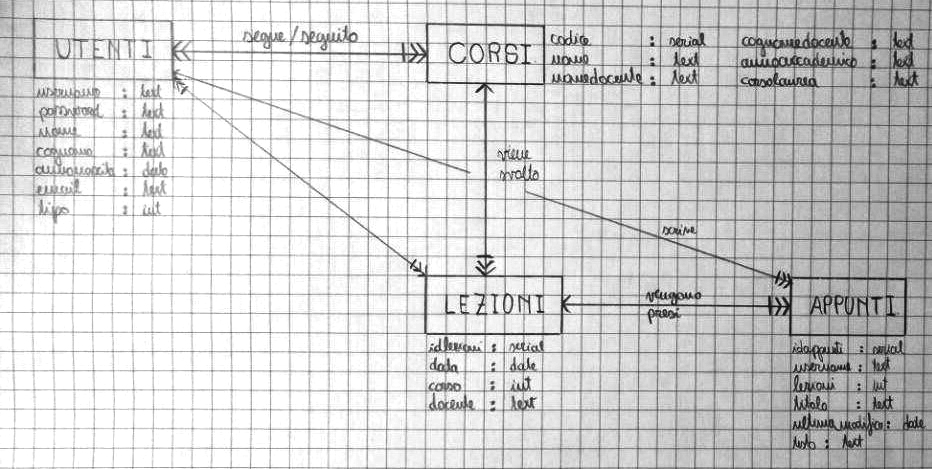
\includegraphics[scale=0.5]{1.jpg}
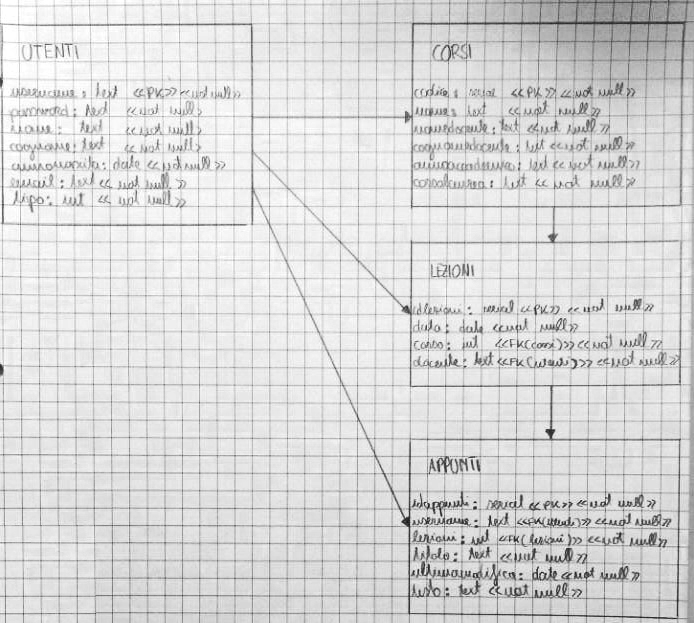
\includegraphics[scale=0.5]{2.jpg}
\end{center}
\chapter{Codice di creazione del database}
\lstinputlisting[language=SQL]{query.sql}
\chapter{Struttura del sito}
\begin{center}
\includegraphics[scale=1.6]{3.jpg}
\end{center}
\chapter{Codice del progetto}
Di seguito, il contenuto di tutti i files del progetto.
\lstinputlisting[language=PHP]{add.php}
\lstinputlisting[language=PHP]{adda.php}
\lstinputlisting[language=PHP]{addappunto.php}
\lstinputlisting[language=PHP]{addcorso.php}
\lstinputlisting[language=PHP]{appunti.php}
\lstinputlisting[language=PHP]{auth.php}
\lstinputlisting[language=PHP]{connessione.php}
\lstinputlisting[language=PHP]{deleteappunto.php}
\lstinputlisting[language=PHP]{deletecorso.php}
\lstinputlisting[language=PHP]{foot.php}
\lstinputlisting[language=PHP]{function.php}
\lstinputlisting[language=PHP]{head.php}
\lstinputlisting[language=PHP]{index.php}
\lstinputlisting[language=PHP]{lezioni.php}
\lstinputlisting[language=PHP]{login.php}
\lstinputlisting[language=PHP]{logout.php}
\lstinputlisting[language=PHP]{newAccount.php}
\lstinputlisting[language=PHP]{phpinfo.php}
\lstinputlisting[language=PHP]{result.php}
\lstinputlisting[language=PHP]{search.php}
\lstinputlisting[language=PHP]{signin.php}
\lstinputlisting[language=PHP]{visualizza.php}
\lstset{inputpath=C:/Users/valdemar/Documents/BasiDiDati/Basi/css}
\lstinputlisting{bootstrap.css}
\lstinputlisting{index.css}
\lstinputlisting{login.css}

\end{document}